\documentclass[8pt,aspectratio=169]{beamer}
%\documentclass[8pt]{beamer}
\usetheme{Montpellier}
\usecolortheme{dove}
\usepackage[utf8]{inputenc}
\usepackage{fontspec} % This line only for XeLaTeX and LuaLaTeX
\usepackage{pgfplots}
\usepackage[english]{babel}
\usepackage{amsmath}
\usepackage{amsfonts}
\usepackage{amssymb}
\usepackage{graphicx}

\usepackage[absolute,overlay]{textpos}

\author{Fabian Schubert}
\title{Learning of Time Sequences through Plasticity in Externally Driven Networks}
%\setbeamercovered{transparent} 
%\setbeamertemplate{navigation symbols}{} 
%\logo{} 
%\institute{} 
\date{18.07.2018} 
%\subject{} 

\begin{document}

\begin{frame}
\titlepage
\end{frame}

\begin{frame}
\tableofcontents
\end{frame}

\section{Introduction to Sequence Learning}
\begin{frame}[t]{What are possible sequence learning tasks?}

\begin{columns}[T]
\begin{column}{0.5\textwidth}
\begin{figure}
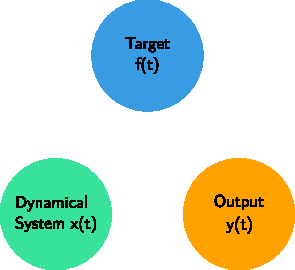
\includegraphics{./figures/sequ_learn_illustration_0.pdf}
\end{figure}
\end{column}
\begin{column}{0.5\textwidth}
How can a dynamical system $x(t)$ be modified appropriately, such that it can generate an output signal $y(t)$ that mimics or predicts some target signal $f(t)$?

In fact, different task scenarios have to be distinguished:

\end{column}
\end{columns}
\end{frame}

\begin{frame}[t]{What are possible sequence learning tasks?}

\begin{columns}[T]
\begin{column}{0.5\textwidth}
\begin{figure}
\begin{picture}(0,0)
\put(-79.9,-130.2){\hbox{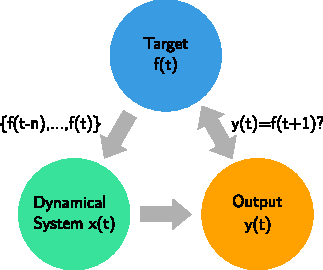
\includegraphics{./figures/sequ_learn_illustration_1.pdf}}}
\end{picture}
\end{figure}
\end{column}
\begin{column}{0.5\textwidth}
How can a dynamical system $x(t)$ be modified appropriately, such that it can generate an output signal $y(t)$ that mimics or predicts some target signal $f(t)$?

In fact, different task scenarios have to be distinguished:

\bigskip
In one scenario, the system is supposed to predict the \emph{future} state of the $f(t)$ based on the history of $f(t)$.

This task usually involves feeding the target signal into the dynamical system, even after learning, since an accurate prediction requires the integration of information about the past.

In this case, the role of the dynamical system can be regarded as a computational, or information processing unit.
\end{column}
\end{columns}
\end{frame}

\begin{frame}[t]{What are possible sequence learning tasks?}

\begin{columns}[T]
\begin{column}{0.5\textwidth}
\begin{figure}
\begin{picture}(0,0)
\put(-71,-130.2){\hbox{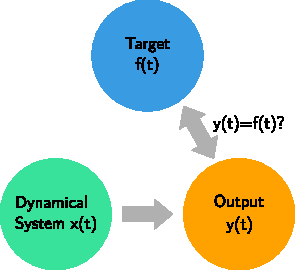
\includegraphics{./figures/sequ_learn_illustration_2.pdf}}}
\end{picture}
\end{figure}
\end{column}
\begin{column}{0.5\textwidth}
How can a dynamical system $x(t)$ be modified appropriately, such that it can generate an output signal $y(t)$ that mimics or predicts some target signal $f(t)$?

In fact, different task scenarios have to be distinguished:

\bigskip
In another case, the dynamical system is supposed to autonomously generate an output $y(t)$ that reproduces $f(t)$.

Here, $x(t)$ does not receive $f(t)$ as an input, since this would turn the task into a trivial problem, solved by simply passing on $f(t)$ to $y(t)$.

In contrast to the first case, the process of learning can be rather interpreted as solely building an internal model of the dynamics underlying $f(t)$.
\end{column}
\end{columns}
\end{frame}

\begin{frame}[t]{What are possible sequence learning tasks?}

\begin{columns}[T]
\begin{column}{0.5\textwidth}
\begin{figure}
\begin{picture}(0,0)
\put(-71,-130.2){\hbox{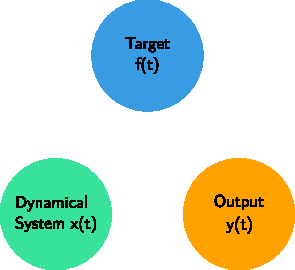
\includegraphics{./figures/sequ_learn_illustration_0.pdf}}}
\end{picture}
\end{figure}
\end{column}
\begin{column}{0.5\textwidth}
Still, also the first tasks requires the system to build some internal representation of the underlying structure of the signal it receives.

In a living organism, the need to autonomously generate patterns of output might seem more ``obvious", e.g. with respect to motor control. However, being able to predict sensory signals is also crucial for taking appropriate actions under a changing environment. 
\end{column}
\end{columns}
\end{frame}


\begin{frame}{Sequence Learning from a Machine Learning Perspective}


\begin{figure}
	\begin{center}
		%% Creator: Matplotlib, PGF backend
%%
%% To include the figure in your LaTeX document, write
%%   \input{<filename>.pgf}
%%
%% Make sure the required packages are loaded in your preamble
%%   \usepackage{pgf}
%%
%% Figures using additional raster images can only be included by \input if
%% they are in the same directory as the main LaTeX file. For loading figures
%% from other directories you can use the `import` package
%%   \usepackage{import}
%% and then include the figures with
%%   \import{<path to file>}{<filename>.pgf}
%%
%% Matplotlib used the following preamble
%%   \usepackage{fontspec}
%%   \setmainfont{DejaVu Serif}
%%   \setsansfont{DejaVu Sans}
%%   \setmonofont{DejaVu Sans Mono}
%%
\begingroup%
\makeatletter%
\begin{pgfpicture}%
\pgfpathrectangle{\pgfpointorigin}{\pgfqpoint{2.800000in}{2.000000in}}%
\pgfusepath{use as bounding box, clip}%
\begin{pgfscope}%
\pgfsetbuttcap%
\pgfsetmiterjoin%
\definecolor{currentfill}{rgb}{1.000000,1.000000,1.000000}%
\pgfsetfillcolor{currentfill}%
\pgfsetlinewidth{0.000000pt}%
\definecolor{currentstroke}{rgb}{1.000000,1.000000,1.000000}%
\pgfsetstrokecolor{currentstroke}%
\pgfsetdash{}{0pt}%
\pgfpathmoveto{\pgfqpoint{0.000000in}{0.000000in}}%
\pgfpathlineto{\pgfqpoint{2.800000in}{0.000000in}}%
\pgfpathlineto{\pgfqpoint{2.800000in}{2.000000in}}%
\pgfpathlineto{\pgfqpoint{0.000000in}{2.000000in}}%
\pgfpathclose%
\pgfusepath{fill}%
\end{pgfscope}%
\begin{pgfscope}%
\pgfsetbuttcap%
\pgfsetmiterjoin%
\definecolor{currentfill}{rgb}{1.000000,1.000000,1.000000}%
\pgfsetfillcolor{currentfill}%
\pgfsetlinewidth{0.000000pt}%
\definecolor{currentstroke}{rgb}{0.000000,0.000000,0.000000}%
\pgfsetstrokecolor{currentstroke}%
\pgfsetstrokeopacity{0.000000}%
\pgfsetdash{}{0pt}%
\pgfpathmoveto{\pgfqpoint{0.350000in}{0.220000in}}%
\pgfpathlineto{\pgfqpoint{2.520000in}{0.220000in}}%
\pgfpathlineto{\pgfqpoint{2.520000in}{1.760000in}}%
\pgfpathlineto{\pgfqpoint{0.350000in}{1.760000in}}%
\pgfpathclose%
\pgfusepath{fill}%
\end{pgfscope}%
\begin{pgfscope}%
\pgfsetbuttcap%
\pgfsetroundjoin%
\definecolor{currentfill}{rgb}{0.000000,0.000000,0.000000}%
\pgfsetfillcolor{currentfill}%
\pgfsetlinewidth{0.803000pt}%
\definecolor{currentstroke}{rgb}{0.000000,0.000000,0.000000}%
\pgfsetstrokecolor{currentstroke}%
\pgfsetdash{}{0pt}%
\pgfsys@defobject{currentmarker}{\pgfqpoint{0.000000in}{-0.048611in}}{\pgfqpoint{0.000000in}{0.000000in}}{%
\pgfpathmoveto{\pgfqpoint{0.000000in}{0.000000in}}%
\pgfpathlineto{\pgfqpoint{0.000000in}{-0.048611in}}%
\pgfusepath{stroke,fill}%
}%
\begin{pgfscope}%
\pgfsys@transformshift{0.448636in}{0.220000in}%
\pgfsys@useobject{currentmarker}{}%
\end{pgfscope}%
\end{pgfscope}%
\begin{pgfscope}%
\pgftext[x=0.448636in,y=0.122778in,,top]{\sffamily\fontsize{8.800000}{10.560000}\selectfont -2}%
\end{pgfscope}%
\begin{pgfscope}%
\pgfsetbuttcap%
\pgfsetroundjoin%
\definecolor{currentfill}{rgb}{0.000000,0.000000,0.000000}%
\pgfsetfillcolor{currentfill}%
\pgfsetlinewidth{0.803000pt}%
\definecolor{currentstroke}{rgb}{0.000000,0.000000,0.000000}%
\pgfsetstrokecolor{currentstroke}%
\pgfsetdash{}{0pt}%
\pgfsys@defobject{currentmarker}{\pgfqpoint{0.000000in}{-0.048611in}}{\pgfqpoint{0.000000in}{0.000000in}}{%
\pgfpathmoveto{\pgfqpoint{0.000000in}{0.000000in}}%
\pgfpathlineto{\pgfqpoint{0.000000in}{-0.048611in}}%
\pgfusepath{stroke,fill}%
}%
\begin{pgfscope}%
\pgfsys@transformshift{0.941818in}{0.220000in}%
\pgfsys@useobject{currentmarker}{}%
\end{pgfscope}%
\end{pgfscope}%
\begin{pgfscope}%
\pgftext[x=0.941818in,y=0.122778in,,top]{\sffamily\fontsize{8.800000}{10.560000}\selectfont -1}%
\end{pgfscope}%
\begin{pgfscope}%
\pgfsetbuttcap%
\pgfsetroundjoin%
\definecolor{currentfill}{rgb}{0.000000,0.000000,0.000000}%
\pgfsetfillcolor{currentfill}%
\pgfsetlinewidth{0.803000pt}%
\definecolor{currentstroke}{rgb}{0.000000,0.000000,0.000000}%
\pgfsetstrokecolor{currentstroke}%
\pgfsetdash{}{0pt}%
\pgfsys@defobject{currentmarker}{\pgfqpoint{0.000000in}{-0.048611in}}{\pgfqpoint{0.000000in}{0.000000in}}{%
\pgfpathmoveto{\pgfqpoint{0.000000in}{0.000000in}}%
\pgfpathlineto{\pgfqpoint{0.000000in}{-0.048611in}}%
\pgfusepath{stroke,fill}%
}%
\begin{pgfscope}%
\pgfsys@transformshift{1.435000in}{0.220000in}%
\pgfsys@useobject{currentmarker}{}%
\end{pgfscope}%
\end{pgfscope}%
\begin{pgfscope}%
\pgftext[x=1.435000in,y=0.122778in,,top]{\sffamily\fontsize{8.800000}{10.560000}\selectfont 0}%
\end{pgfscope}%
\begin{pgfscope}%
\pgfsetbuttcap%
\pgfsetroundjoin%
\definecolor{currentfill}{rgb}{0.000000,0.000000,0.000000}%
\pgfsetfillcolor{currentfill}%
\pgfsetlinewidth{0.803000pt}%
\definecolor{currentstroke}{rgb}{0.000000,0.000000,0.000000}%
\pgfsetstrokecolor{currentstroke}%
\pgfsetdash{}{0pt}%
\pgfsys@defobject{currentmarker}{\pgfqpoint{0.000000in}{-0.048611in}}{\pgfqpoint{0.000000in}{0.000000in}}{%
\pgfpathmoveto{\pgfqpoint{0.000000in}{0.000000in}}%
\pgfpathlineto{\pgfqpoint{0.000000in}{-0.048611in}}%
\pgfusepath{stroke,fill}%
}%
\begin{pgfscope}%
\pgfsys@transformshift{1.928182in}{0.220000in}%
\pgfsys@useobject{currentmarker}{}%
\end{pgfscope}%
\end{pgfscope}%
\begin{pgfscope}%
\pgftext[x=1.928182in,y=0.122778in,,top]{\sffamily\fontsize{8.800000}{10.560000}\selectfont 1}%
\end{pgfscope}%
\begin{pgfscope}%
\pgfsetbuttcap%
\pgfsetroundjoin%
\definecolor{currentfill}{rgb}{0.000000,0.000000,0.000000}%
\pgfsetfillcolor{currentfill}%
\pgfsetlinewidth{0.803000pt}%
\definecolor{currentstroke}{rgb}{0.000000,0.000000,0.000000}%
\pgfsetstrokecolor{currentstroke}%
\pgfsetdash{}{0pt}%
\pgfsys@defobject{currentmarker}{\pgfqpoint{0.000000in}{-0.048611in}}{\pgfqpoint{0.000000in}{0.000000in}}{%
\pgfpathmoveto{\pgfqpoint{0.000000in}{0.000000in}}%
\pgfpathlineto{\pgfqpoint{0.000000in}{-0.048611in}}%
\pgfusepath{stroke,fill}%
}%
\begin{pgfscope}%
\pgfsys@transformshift{2.421364in}{0.220000in}%
\pgfsys@useobject{currentmarker}{}%
\end{pgfscope}%
\end{pgfscope}%
\begin{pgfscope}%
\pgftext[x=2.421364in,y=0.122778in,,top]{\sffamily\fontsize{8.800000}{10.560000}\selectfont 2}%
\end{pgfscope}%
\begin{pgfscope}%
\pgfsetbuttcap%
\pgfsetroundjoin%
\definecolor{currentfill}{rgb}{0.000000,0.000000,0.000000}%
\pgfsetfillcolor{currentfill}%
\pgfsetlinewidth{0.803000pt}%
\definecolor{currentstroke}{rgb}{0.000000,0.000000,0.000000}%
\pgfsetstrokecolor{currentstroke}%
\pgfsetdash{}{0pt}%
\pgfsys@defobject{currentmarker}{\pgfqpoint{-0.048611in}{0.000000in}}{\pgfqpoint{0.000000in}{0.000000in}}{%
\pgfpathmoveto{\pgfqpoint{0.000000in}{0.000000in}}%
\pgfpathlineto{\pgfqpoint{-0.048611in}{0.000000in}}%
\pgfusepath{stroke,fill}%
}%
\begin{pgfscope}%
\pgfsys@transformshift{0.350000in}{0.289999in}%
\pgfsys@useobject{currentmarker}{}%
\end{pgfscope}%
\end{pgfscope}%
\begin{pgfscope}%
\pgftext[x=0.175016in,y=0.243568in,left,base]{\sffamily\fontsize{8.800000}{10.560000}\selectfont 0}%
\end{pgfscope}%
\begin{pgfscope}%
\pgfsetbuttcap%
\pgfsetroundjoin%
\definecolor{currentfill}{rgb}{0.000000,0.000000,0.000000}%
\pgfsetfillcolor{currentfill}%
\pgfsetlinewidth{0.803000pt}%
\definecolor{currentstroke}{rgb}{0.000000,0.000000,0.000000}%
\pgfsetstrokecolor{currentstroke}%
\pgfsetdash{}{0pt}%
\pgfsys@defobject{currentmarker}{\pgfqpoint{-0.048611in}{0.000000in}}{\pgfqpoint{0.000000in}{0.000000in}}{%
\pgfpathmoveto{\pgfqpoint{0.000000in}{0.000000in}}%
\pgfpathlineto{\pgfqpoint{-0.048611in}{0.000000in}}%
\pgfusepath{stroke,fill}%
}%
\begin{pgfscope}%
\pgfsys@transformshift{0.350000in}{0.639999in}%
\pgfsys@useobject{currentmarker}{}%
\end{pgfscope}%
\end{pgfscope}%
\begin{pgfscope}%
\pgftext[x=0.175016in,y=0.593569in,left,base]{\sffamily\fontsize{8.800000}{10.560000}\selectfont 1}%
\end{pgfscope}%
\begin{pgfscope}%
\pgfsetbuttcap%
\pgfsetroundjoin%
\definecolor{currentfill}{rgb}{0.000000,0.000000,0.000000}%
\pgfsetfillcolor{currentfill}%
\pgfsetlinewidth{0.803000pt}%
\definecolor{currentstroke}{rgb}{0.000000,0.000000,0.000000}%
\pgfsetstrokecolor{currentstroke}%
\pgfsetdash{}{0pt}%
\pgfsys@defobject{currentmarker}{\pgfqpoint{-0.048611in}{0.000000in}}{\pgfqpoint{0.000000in}{0.000000in}}{%
\pgfpathmoveto{\pgfqpoint{0.000000in}{0.000000in}}%
\pgfpathlineto{\pgfqpoint{-0.048611in}{0.000000in}}%
\pgfusepath{stroke,fill}%
}%
\begin{pgfscope}%
\pgfsys@transformshift{0.350000in}{0.989999in}%
\pgfsys@useobject{currentmarker}{}%
\end{pgfscope}%
\end{pgfscope}%
\begin{pgfscope}%
\pgftext[x=0.175016in,y=0.943569in,left,base]{\sffamily\fontsize{8.800000}{10.560000}\selectfont 2}%
\end{pgfscope}%
\begin{pgfscope}%
\pgfsetbuttcap%
\pgfsetroundjoin%
\definecolor{currentfill}{rgb}{0.000000,0.000000,0.000000}%
\pgfsetfillcolor{currentfill}%
\pgfsetlinewidth{0.803000pt}%
\definecolor{currentstroke}{rgb}{0.000000,0.000000,0.000000}%
\pgfsetstrokecolor{currentstroke}%
\pgfsetdash{}{0pt}%
\pgfsys@defobject{currentmarker}{\pgfqpoint{-0.048611in}{0.000000in}}{\pgfqpoint{0.000000in}{0.000000in}}{%
\pgfpathmoveto{\pgfqpoint{0.000000in}{0.000000in}}%
\pgfpathlineto{\pgfqpoint{-0.048611in}{0.000000in}}%
\pgfusepath{stroke,fill}%
}%
\begin{pgfscope}%
\pgfsys@transformshift{0.350000in}{1.340000in}%
\pgfsys@useobject{currentmarker}{}%
\end{pgfscope}%
\end{pgfscope}%
\begin{pgfscope}%
\pgftext[x=0.175016in,y=1.293570in,left,base]{\sffamily\fontsize{8.800000}{10.560000}\selectfont 3}%
\end{pgfscope}%
\begin{pgfscope}%
\pgfsetbuttcap%
\pgfsetroundjoin%
\definecolor{currentfill}{rgb}{0.000000,0.000000,0.000000}%
\pgfsetfillcolor{currentfill}%
\pgfsetlinewidth{0.803000pt}%
\definecolor{currentstroke}{rgb}{0.000000,0.000000,0.000000}%
\pgfsetstrokecolor{currentstroke}%
\pgfsetdash{}{0pt}%
\pgfsys@defobject{currentmarker}{\pgfqpoint{-0.048611in}{0.000000in}}{\pgfqpoint{0.000000in}{0.000000in}}{%
\pgfpathmoveto{\pgfqpoint{0.000000in}{0.000000in}}%
\pgfpathlineto{\pgfqpoint{-0.048611in}{0.000000in}}%
\pgfusepath{stroke,fill}%
}%
\begin{pgfscope}%
\pgfsys@transformshift{0.350000in}{1.690000in}%
\pgfsys@useobject{currentmarker}{}%
\end{pgfscope}%
\end{pgfscope}%
\begin{pgfscope}%
\pgftext[x=0.175016in,y=1.643570in,left,base]{\sffamily\fontsize{8.800000}{10.560000}\selectfont 4}%
\end{pgfscope}%
\begin{pgfscope}%
\pgfpathrectangle{\pgfqpoint{0.350000in}{0.220000in}}{\pgfqpoint{2.170000in}{1.540000in}}%
\pgfusepath{clip}%
\pgfsetrectcap%
\pgfsetroundjoin%
\pgfsetlinewidth{1.505625pt}%
\definecolor{currentstroke}{rgb}{0.121569,0.466667,0.705882}%
\pgfsetstrokecolor{currentstroke}%
\pgfsetdash{}{0pt}%
\pgfpathmoveto{\pgfqpoint{0.448636in}{1.690000in}}%
\pgfpathlineto{\pgfqpoint{0.496029in}{1.558697in}}%
\pgfpathlineto{\pgfqpoint{0.543422in}{1.433859in}}%
\pgfpathlineto{\pgfqpoint{0.588840in}{1.320288in}}%
\pgfpathlineto{\pgfqpoint{0.634258in}{1.212653in}}%
\pgfpathlineto{\pgfqpoint{0.677702in}{1.115254in}}%
\pgfpathlineto{\pgfqpoint{0.721145in}{1.023286in}}%
\pgfpathlineto{\pgfqpoint{0.762614in}{0.940565in}}%
\pgfpathlineto{\pgfqpoint{0.804083in}{0.862794in}}%
\pgfpathlineto{\pgfqpoint{0.843577in}{0.793327in}}%
\pgfpathlineto{\pgfqpoint{0.883071in}{0.728349in}}%
\pgfpathlineto{\pgfqpoint{0.920590in}{0.670778in}}%
\pgfpathlineto{\pgfqpoint{0.958109in}{0.617258in}}%
\pgfpathlineto{\pgfqpoint{0.993654in}{0.570292in}}%
\pgfpathlineto{\pgfqpoint{1.029199in}{0.526962in}}%
\pgfpathlineto{\pgfqpoint{1.062769in}{0.489378in}}%
\pgfpathlineto{\pgfqpoint{1.096339in}{0.455037in}}%
\pgfpathlineto{\pgfqpoint{1.129909in}{0.423940in}}%
\pgfpathlineto{\pgfqpoint{1.161504in}{0.397634in}}%
\pgfpathlineto{\pgfqpoint{1.193099in}{0.374202in}}%
\pgfpathlineto{\pgfqpoint{1.224694in}{0.353642in}}%
\pgfpathlineto{\pgfqpoint{1.254315in}{0.336977in}}%
\pgfpathlineto{\pgfqpoint{1.283935in}{0.322837in}}%
\pgfpathlineto{\pgfqpoint{1.313556in}{0.311222in}}%
\pgfpathlineto{\pgfqpoint{1.341202in}{0.302659in}}%
\pgfpathlineto{\pgfqpoint{1.368847in}{0.296296in}}%
\pgfpathlineto{\pgfqpoint{1.396493in}{0.292132in}}%
\pgfpathlineto{\pgfqpoint{1.424139in}{0.290168in}}%
\pgfpathlineto{\pgfqpoint{1.451785in}{0.290404in}}%
\pgfpathlineto{\pgfqpoint{1.479431in}{0.292839in}}%
\pgfpathlineto{\pgfqpoint{1.507077in}{0.297474in}}%
\pgfpathlineto{\pgfqpoint{1.534722in}{0.304309in}}%
\pgfpathlineto{\pgfqpoint{1.562368in}{0.313343in}}%
\pgfpathlineto{\pgfqpoint{1.591989in}{0.325463in}}%
\pgfpathlineto{\pgfqpoint{1.621609in}{0.340108in}}%
\pgfpathlineto{\pgfqpoint{1.651230in}{0.357279in}}%
\pgfpathlineto{\pgfqpoint{1.680850in}{0.376974in}}%
\pgfpathlineto{\pgfqpoint{1.712446in}{0.400766in}}%
\pgfpathlineto{\pgfqpoint{1.744041in}{0.427430in}}%
\pgfpathlineto{\pgfqpoint{1.775636in}{0.456968in}}%
\pgfpathlineto{\pgfqpoint{1.809206in}{0.491499in}}%
\pgfpathlineto{\pgfqpoint{1.842776in}{0.529274in}}%
\pgfpathlineto{\pgfqpoint{1.876346in}{0.570292in}}%
\pgfpathlineto{\pgfqpoint{1.911891in}{0.617258in}}%
\pgfpathlineto{\pgfqpoint{1.947435in}{0.667860in}}%
\pgfpathlineto{\pgfqpoint{1.984954in}{0.725218in}}%
\pgfpathlineto{\pgfqpoint{2.022474in}{0.786627in}}%
\pgfpathlineto{\pgfqpoint{2.061968in}{0.855645in}}%
\pgfpathlineto{\pgfqpoint{2.101462in}{0.929152in}}%
\pgfpathlineto{\pgfqpoint{2.142931in}{1.011166in}}%
\pgfpathlineto{\pgfqpoint{2.184399in}{1.098128in}}%
\pgfpathlineto{\pgfqpoint{2.227843in}{1.194540in}}%
\pgfpathlineto{\pgfqpoint{2.271286in}{1.296384in}}%
\pgfpathlineto{\pgfqpoint{2.316704in}{1.408665in}}%
\pgfpathlineto{\pgfqpoint{2.362123in}{1.526882in}}%
\pgfpathlineto{\pgfqpoint{2.409515in}{1.656568in}}%
\pgfpathlineto{\pgfqpoint{2.421364in}{1.690000in}}%
\pgfpathlineto{\pgfqpoint{2.421364in}{1.690000in}}%
\pgfusepath{stroke}%
\end{pgfscope}%
\begin{pgfscope}%
\pgfsetrectcap%
\pgfsetmiterjoin%
\pgfsetlinewidth{0.803000pt}%
\definecolor{currentstroke}{rgb}{0.000000,0.000000,0.000000}%
\pgfsetstrokecolor{currentstroke}%
\pgfsetdash{}{0pt}%
\pgfpathmoveto{\pgfqpoint{0.350000in}{0.220000in}}%
\pgfpathlineto{\pgfqpoint{0.350000in}{1.760000in}}%
\pgfusepath{stroke}%
\end{pgfscope}%
\begin{pgfscope}%
\pgfsetrectcap%
\pgfsetmiterjoin%
\pgfsetlinewidth{0.803000pt}%
\definecolor{currentstroke}{rgb}{0.000000,0.000000,0.000000}%
\pgfsetstrokecolor{currentstroke}%
\pgfsetdash{}{0pt}%
\pgfpathmoveto{\pgfqpoint{2.520000in}{0.220000in}}%
\pgfpathlineto{\pgfqpoint{2.520000in}{1.760000in}}%
\pgfusepath{stroke}%
\end{pgfscope}%
\begin{pgfscope}%
\pgfsetrectcap%
\pgfsetmiterjoin%
\pgfsetlinewidth{0.803000pt}%
\definecolor{currentstroke}{rgb}{0.000000,0.000000,0.000000}%
\pgfsetstrokecolor{currentstroke}%
\pgfsetdash{}{0pt}%
\pgfpathmoveto{\pgfqpoint{0.350000in}{0.220000in}}%
\pgfpathlineto{\pgfqpoint{2.520000in}{0.220000in}}%
\pgfusepath{stroke}%
\end{pgfscope}%
\begin{pgfscope}%
\pgfsetrectcap%
\pgfsetmiterjoin%
\pgfsetlinewidth{0.803000pt}%
\definecolor{currentstroke}{rgb}{0.000000,0.000000,0.000000}%
\pgfsetstrokecolor{currentstroke}%
\pgfsetdash{}{0pt}%
\pgfpathmoveto{\pgfqpoint{0.350000in}{1.760000in}}%
\pgfpathlineto{\pgfqpoint{2.520000in}{1.760000in}}%
\pgfusepath{stroke}%
\end{pgfscope}%
\begin{pgfscope}%
\pgftext[x=1.435000in,y=1.843333in,,base]{\sffamily\fontsize{10.560000}{12.672000}\selectfont This is a text}%
\end{pgfscope}%
\end{pgfpicture}%
\makeatother%
\endgroup%

	\end{center}
\end{figure}



\end{frame}


\end{document}